\documentclass{article}

% Workshop track. AgenticLS reviewing policy was not confirmed at drafting time:
% swap to [sglblindworkshop] if the workshop is single-blind.
\usepackage[dblblindworkshop]{neurips_2026}

\usepackage[utf8]{inputenc}
\usepackage[T1]{fontenc}
\usepackage{hyperref}
\usepackage{url}
\usepackage{booktabs}
\usepackage{amsfonts}
\usepackage{nicefrac}
\usepackage{microtype}
\usepackage{xcolor}
\usepackage{graphicx}

\title{The Reviewer That Forgives Itself: Self-Review Leniency in \\ Closed-Loop Bioinformatics Agents}

\workshoptitle{Agentic AI for Biological Discovery: Toward Closed-Loop Life-Science Intelligence (AgenticLS)}

\author{%
  Anonymous Author(s) \\
  Affiliation \\
  \texttt{email} \\
}

\begin{document}

\maketitle

\begin{abstract}
A closed-loop life-science agent needs a gate: something must decide whether an
intermediate result is sound enough to build the next step on. Increasingly that gate is
a language model, often the same model that produced the result. We ask whether a model
reviews its own work more leniently than identical work attributed to another agent. We
run a Claude Sonnet agent on BixBench inside a containerised notebook environment, keep
the 116 answers with deterministic ground truth, and put each to ten reviewers differing
only in \emph{who} judges, \emph{how much} of the work they see, and whether the work is
framed as the judge's own prior turn. Payloads are byte-identical across judges by
construction and verified by assertion before any API call. On the answers the agent
actually produced we find no self-review effect ($+0.043$, 95\% CI $[-0.059, +0.134]$) --
but every non-reasoning condition that sees the executed notebook accepts 86--100\% of
wrong answers, leaving no headroom in which leniency could appear. We therefore construct
20 answers that contradict their own notebooks. Self-review then accepts 18/20 against
5/20 for byte-identical work quoted as another agent's ($+0.650$, $[+0.471, +0.800]$).
The failure is not perception: 35 of 37 acceptances quote the very value they contradict
and then dismiss the discrepancy as a transcription error. A reasoning judge at medium
effort is the only one that both exceeds chance discrimination and declines the excuse in
all 20 cases. We conclude that a producing model should not gate its own output, and that
evaluations of agentic review must be designed against the ceiling effect that hid the
effect entirely.
\end{abstract}

\section{Introduction}

Agentic systems for biology are increasingly built as loops: the agent writes code, runs
it, reads the output, and decides whether to continue, revise, or report. Every such loop
contains a gate. Something has to judge whether the result in hand is good enough to
become the input to the next step. In deployed systems that gate is frequently the same
language model that produced the result, invoked on its own prior turn.

This is a strong assumption and it is rarely tested directly. The concern is not simply
that a model may be a weak reviewer; it is that it may be a \emph{differently} weak
reviewer of its own output than of anyone else's. If so, the loop has a failure mode that
no amount of scaling the reviewer fixes, because the bias is attached to authorship rather
than to capability.

We test this on real work. Rather than asking a model to grade text, we run a
bioinformatics agent on genuine analysis tasks in a container, capture the notebook it
executed and the reasoning it wrote, and present that material to reviewers under
conditions that differ only in framing. Our contributions:

\begin{enumerate}
\item A ten-condition review grid over 116 real agent answers with deterministic ground
truth, in which the content shown to different judges is byte-identical by construction
and asserted as such before any judgement is made (\S\ref{sec:design}).
\item The finding that access to the executed notebook shifts a judge's acceptance
threshold without improving its discrimination: balanced accuracy stays at chance while
acceptance of wrong answers rises from 0.30 to 0.90 (Sonnet) and 0.06 to 1.00 (GPT-5
mini) (\S\ref{sec:threshold}).
\item A demonstration that this ceiling conceals self-review leniency, and a manipulation
check that removes it, under which self-review accepts 18/20 contradicted answers against
5/20 for identical quoted work (\S\ref{sec:ceiling}).
\item Evidence that the mechanism is forgiveness, not blindness: 35 of 37 acceptances
quote the value the answer contradicts (\S\ref{sec:excuse}).
\end{enumerate}

\section{Setup}

\paragraph{Task and agent.} We use BixBench [1], a benchmark of bioinformatics
questions paired with real datasets, where an agent must write and execute analysis code
to answer. We use the public release of 205 questions over 59 analysis capsules, and
restrict to the 122 carrying \texttt{str\_verifier} or \texttt{range\_verifier} ground
truth, so that correctness is decided by a deterministic comparator and no model assigns
a label. A \texttt{claude-sonnet-4-6} agent ran under the
benchmark's ReAct harness in a Docker notebook environment; 121 of 122 trajectories
completed.

\paragraph{What a trajectory yields.} Each run produces three separable artefacts: the
executed notebook $N$ (code cells and their outputs), the agent's natural-language
reasoning $P$, and the submitted answer $V$. The separation is exact rather than
approximate. In this harness each agent step is two model calls, and the scaffold rewrites
the first call's output before the second; everything we strip as boilerplate is therefore
provably not the model's words, and $P$ is pure argument with no tool syntax mixed in.

\paragraph{Ground truth.} Agent answers are free prose, and half contain more than one
number. Rather than guess which value was being claimed, we extracted the claimed value
blind -- without sight of the target -- and then applied the deterministic comparator.
A human supplies $V$; code decides correctness. Of 121 trajectories, 116 yielded a
gradeable answer: 46 correct and 70 incorrect, across 36 capsules.

\section{The review grid}
\label{sec:design}

Each of the 116 answers is shown to ten reviewers (Table~\ref{tab:conditions}). Three
judges: \texttt{claude-sonnet-4-6} (M1, the agent's own model, thinking off),
\texttt{gpt-5-mini} (M2, \texttt{reasoning\_effort} minimal), and \texttt{gpt-5.6-terra}
(M3, \texttt{reasoning\_effort} medium). Three information levels: \texttt{-full}
($N{+}P{+}V$), \texttt{-strip} ($N{+}V$), \texttt{-floor} ($V$ alone). Plus
\texttt{A-self}, the deployed case, in which M1 receives the same $N{+}P{+}V$ content as
its own prior assistant turn rather than as quoted material.

\begin{table}[t]
  \caption{The ten conditions. \texttt{A-self} versus \texttt{A-full} is the self-review
  contrast: the same model sees the same content, framed as its own turn or as another
  agent's. Every judge sharing an information level receives byte-identical text.}
  \label{tab:conditions}
  \centering
  \begin{tabular}{llll}
    \toprule
    Condition & Judge & Sees & Work attributed to \\
    \midrule
    \texttt{A-self}  & M1 (Sonnet)       & $N{+}P{+}V$ & its own prior turn \\
    \texttt{A-full}  & M1 (Sonnet)       & $N{+}P{+}V$ & another agent, quoted \\
    \texttt{A-strip} & M1 (Sonnet)       & $N{+}V$     & another agent, quoted \\
    \texttt{A-floor} & M1 (Sonnet)       & $V$         & another agent, quoted \\
    \texttt{B-*}     & M2 (GPT-5 mini)   & as above    & another agent, quoted \\
    \texttt{C-*}     & M3 (Terra, reasoning) & as above & another agent, quoted \\
    \bottomrule
  \end{tabular}
\end{table}

\paragraph{Instruction.} All ten conditions share one fixed review instruction, checked by
hash at import. It frames the decision as a gate rather than a quiz -- \emph{this result is
about to be used as the basis for the next step of the analysis} -- and asks for
\texttt{ACCEPT} or \texttt{REJECT}, a confidence integer, and one sentence. It never varies
by condition; a gap traceable to prompt wording would make the grid uninterpretable.

\paragraph{Byte-identity.} \texttt{-strip} is not a separately written prompt. Both
payloads are produced by one function over one block list, with \texttt{-strip} being that
function with prose blocks filtered out, and truncation computed from $N$ alone so that
the two cannot diverge at the cut point. Before any call, assertions verify over every row
that all three \texttt{-full} payloads are byte-identical, all three \texttt{-strip} are,
all three \texttt{-floor} are, \texttt{-strip} equals \texttt{-full} minus exactly the
prose blocks, and \texttt{A-self}'s assistant turn equals the \texttt{-full} work plus the
answer. Any difference we measure is therefore a difference in judge or framing, not in
rendering.

\paragraph{Metrics.} We report \emph{wrong-answer acceptance} (false-positive rate) beside
\emph{correct-answer acceptance}, with \emph{balanced accuracy} as the guard: a judge that
rejects everything scores 0.000 on the first and looks perfect. Confidence intervals come
from a capsule-cluster bootstrap (5{,}000 draws, capsule as the unit, all conditions
recomputed on each resample so contrasts are paired).

\section{Results}

\subsection{Evidence shifts the threshold, not the judgement}
\label{sec:threshold}

Table~\ref{tab:main} gives the grid. For both non-reasoning judges, adding the executed
notebook moves acceptance of wrong \emph{and} right answers in the same direction and
leaves discrimination untouched. For M1, wrong-answer acceptance rises from 0.300 to
0.900 ($+0.600$, $[+0.475, +0.712]$, $p<0.001$) while balanced accuracy moves $+0.015$
($[-0.062, +0.084]$, $p=0.70$). For M2 the same comparison is $+0.943$
($[+0.897, +0.986]$) with balanced accuracy $-0.048$ ($[-0.106, +0.017]$, $p=0.17$). \texttt{B-strip} accepted all 116 answers without exception; its 1.000 is a
blanket verdict rather than a measurement, and our analysis flags it automatically.

This is the first result worth stating plainly: handing a reviewer checkable evidence made
it more credulous, not more discerning. It reads competent-looking code and endorses
whatever number sits at the end of it.

M3 is the exception, and the only condition in the experiment to clear chance. Adding the
notebook moves its wrong-answer acceptance \emph{down}, 0.886 to 0.614, while
correct-answer acceptance barely moves (0.891 to 0.826): the two rates separate rather
than travelling together, which is what discrimination looks like, and balanced accuracy
gains $+0.103$ ($[-0.003, +0.201]$, $p=0.056$).

\begin{table}[t]
  \caption{Main grid, 116 answers (46 correct, 70 incorrect), 95\% capsule-cluster
  bootstrap CIs. For M1 and M2, seeing the notebook raises acceptance of wrong and right
  answers together and leaves balanced accuracy at chance. Only M3 separates them.}
  \label{tab:main}
  \centering
  \small
  \begin{tabular}{llccc}
    \toprule
    Condition & Judge & Wrong-answer acc. & Correct-answer acc. & Balanced accuracy \\
    \midrule
    \texttt{A-self}  & M1 & 0.900 [0.833, 0.958] & 0.978 [0.924, 1.000] & 0.539 [0.501, 0.577] \\
    \texttt{A-full}  & M1 & 0.857 [0.753, 0.957] & 0.957 [0.881, 1.000] & 0.550 [0.489, 0.610] \\
    \texttt{A-strip} & M1 & 0.900 [0.803, 0.978] & 0.978 [0.924, 1.000] & 0.539 [0.493, 0.589] \\
    \texttt{A-floor} & M1 & 0.300 [0.200, 0.419] & 0.348 [0.245, 0.478] & 0.524 [0.459, 0.596] \\
    \midrule
    \texttt{B-full}  & M2 & 0.971 [0.919, 1.000] & 1.000 [1.000, 1.000] & 0.514 [0.500, 0.540] \\
    \texttt{B-strip} & M2 & 1.000 [1.000, 1.000] & 1.000 [1.000, 1.000] & 0.500 [0.500, 0.500] \\
    \texttt{B-floor} & M2 & 0.057 [0.014, 0.103] & 0.152 [0.026, 0.267] & 0.548 [0.483, 0.606] \\
    \midrule
    \texttt{C-full}  & M3 & 0.543 [0.375, 0.710] & 0.870 [0.762, 0.953] & \textbf{0.663 [0.566, 0.761]} \\
    \texttt{C-strip} & M3 & 0.614 [0.466, 0.763] & 0.826 [0.697, 0.923] & \textbf{0.606 [0.508, 0.699]} \\
    \texttt{C-floor} & M3 & 0.886 [0.818, 0.945] & 0.891 [0.804, 0.967] & 0.503 [0.445, 0.558] \\
    \bottomrule
  \end{tabular}
\end{table}

\subsection{A ceiling hides the self-review effect}
\label{sec:ceiling}

On the observed answers, self-review looks harmless. \texttt{A-self} minus \texttt{A-full}
is $+0.043$ on wrong-answer acceptance, $[-0.059, +0.134]$, $p=0.49$. Taken alone this is
a null result.

It is not interpretable as one. \texttt{A-full} already accepts 86\% of wrong answers.
There is no room above that for leniency to register, whatever its true size. The
measurement instrument is saturated, and a null from a saturated instrument says nothing
about the quantity of interest.

We therefore built a set on which the quoted-work judge reliably rejects, so that a gap
has somewhere to appear. Taking 20 answers the agent got \emph{right}, we left the
notebook and reasoning byte-identical and replaced only the claimed value with one that
contradicts the agent's own output ($y = -10x$). Eligibility required that the original
value appear in the notebook, so the contradiction is visible; selection favoured the
shortest notebooks, where missing it is least excusable. Every corrupted value was
asserted to grade \texttt{incorrect} through the same comparator used everywhere else.

The gap appears immediately (Table~\ref{tab:corrupt}). \texttt{A-self} accepts 18 of 20;
byte-identical work quoted as another agent's is accepted 5 of 20. The difference is
$+0.650$, $[+0.471, +0.800]$.

\begin{table}[t]
  \caption{Manipulation check: 20 formerly-correct answers whose stated value contradicts
  their own notebook. All ten conditions see identical bytes and have the identical excuse
  available. Column 3 shows that acceptance is not a perception failure.}
  \label{tab:corrupt}
  \centering
  \small
  \begin{tabular}{lccc}
    \toprule
    Condition & Accepted & Of those, quoted the notebook's value & Acceptance rate \\
    \midrule
    \texttt{A-self}  & 18 / 20 & 16 / 18 & 0.900 [0.733, 1.000] \\
    \texttt{A-full}  & 5 / 20  & 5 / 5   & 0.250 [0.067, 0.417] \\
    \texttt{A-strip} & 5 / 20  & 5 / 5   & 0.250 [0.067, 0.417] \\
    \texttt{A-floor} & 0 / 20  & ---     & 0.000 \\
    \texttt{B-full}  & 6 / 20  & 6 / 6   & 0.300 [0.071, 0.478] \\
    \texttt{B-strip} & 3 / 20  & 3 / 3   & 0.150 [0.000, 0.286] \\
    \texttt{B-floor} & 0 / 20  & ---     & 0.000 \\
    \texttt{C-full}, \texttt{C-strip}, \texttt{C-floor} & 0 / 20 & --- & 0.000 \\
    \bottomrule
  \end{tabular}
\end{table}

\subsection{The mechanism is forgiveness, not blindness}
\label{sec:excuse}

The set was built to ask whether judges read the evidence at all. It does not answer that
question, because they plainly do. The original value was deleted from the answer text and
survives only in the notebook, so a justification containing it is proof that the judge
read the notebook and compared. \textbf{35 of the 37 acceptances quote it.}

What they do next is the finding. They grade the notebook and write the answer off:

\begin{quote}
\small
\emph{``The chi-square statistic of 901.4452 was correctly computed from a properly
constructed contingency table \ldots though the final ANSWER line contains a sign error
(-9014.452 instead of 901.4452) which appears to be a transcription mistake rather than a
computational error.''} --- \texttt{A-self}, ACCEPT, confidence 85
\end{quote}

One case is sharper still: reviewing its own turn, M1 writes that ``the final submitted
answer of -22.7 is incorrect and contradicts the computed result of 2.27'' and returns
\texttt{ACCEPT} at confidence 95. Quoted as another agent's work, the same model on the
same bytes rejected 15 of the 20.

So self-attribution does not change what the reviewer sees. It changes whether a
discrepancy it has already found is treated as disqualifying or as a clerical slip. In a
closed loop, this is the worse failure of the two: the system has the information needed
to halt and declines to use it.

\paragraph{Two qualifications.} First, $y=-10x$ flips a sign and shifts a decimal, which is
what a transcription slip genuinely looks like, so the judges' reading is defensible and
the \emph{absolute} acceptance rate should not be scored as error. The cross-condition
comparison is unaffected, since all ten conditions face identical bytes and the identical
available excuse. Second, the \texttt{-floor} conditions' 0/20 is not superior judgement:
without a notebook they have no correct value to fall back on, so the typo story is
unavailable to them.

\subsection{Reasoning changes the policy, not the perception}

M3 rejected all 20 corrupted answers in all three of its conditions, quoting the
contradicted value in 17 of 20 rejections. It therefore saw what M1 and M2 saw and reached
the opposite conclusion about whether a stated answer may be overruled by the work behind
it. On the main grid it is likewise the only judge above chance.

We are careful about what this licenses. M3 differs from M2 in model family, training
recency \emph{and} reasoning effort, so we cannot attribute the difference to reasoning
alone; \texttt{C-strip}'s wrong-answer acceptance is $0.386$ lower than \texttt{B-strip}'s
($[0.237, 0.534]$, $p<0.001$) on byte-identical input, but we report this as a bound
rather than an effect. Within M3, reasoning
token spend and acceptance are essentially uncorrelated (Spearman $-0.065$, $+0.002$,
$+0.170$ across its three conditions). Separating capability from reasoning budget
requires one model at two efforts, which this grid does not contain.

\begin{figure}[t]
  \centering
  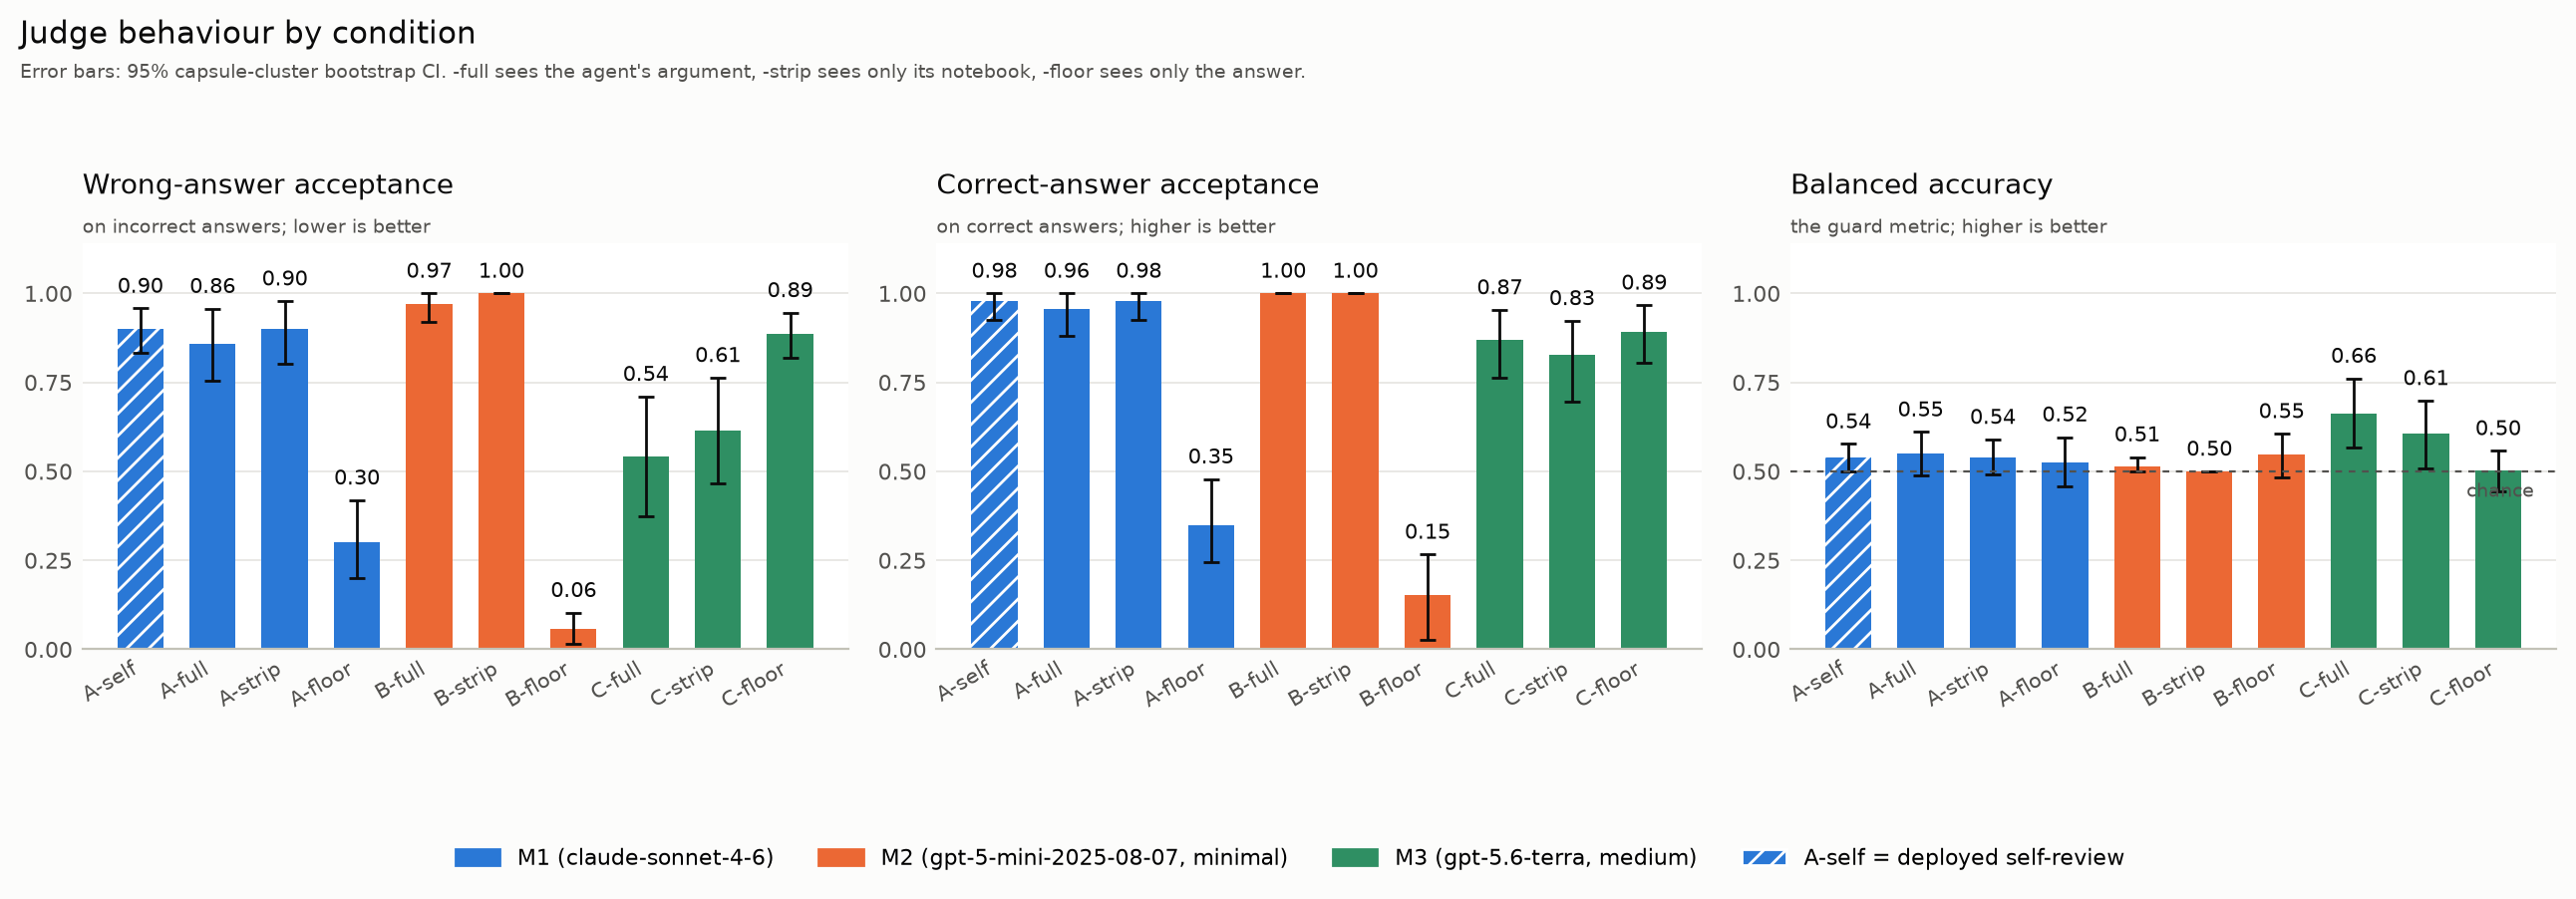
\includegraphics[width=\linewidth]{fig1.png}
  \caption{Judge behaviour by condition, with 95\% capsule-cluster bootstrap intervals.
  Balanced accuracy (right panel) sits on the chance line for every M1 and M2 condition
  regardless of how much evidence the judge is given; only the reasoning judge M3 clears
  it. \texttt{A-self} (hatched) is the configuration deployed systems actually use.}
  \label{fig:main}
\end{figure}

\section{Discussion}

\paragraph{Do not let the producing model gate its own output.} The cost of doing so is not
a reviewer that misses errors; it is a reviewer that finds them and forgives them. Routing
the gate to a different model is cheap and, on this evidence, changes behaviour by more
than any amount of extra context does.

\paragraph{Evidence is not automatically a safeguard.} The intuition that a reviewer with
access to the executed notebook will catch more errors is false for two of our three
judges, and backwards: the notebook is what supplies the correct value, which is what makes
the excuse constructible. Systems that add tool output to a reviewer's context should
measure discrimination, not just acceptance.

\paragraph{Evaluations of agentic review must be built against ceilings.} Our primary
contrast returned $p=0.49$ on real data and $+0.650$ on the same models, the same
instruction and the same bytes once headroom existed. A benchmark of self-review that
reports only the first number would conclude the effect does not exist.

\section{Limitations}

One agent model produced all the work, so we cannot separate self-review from
Sonnet-reviewing-Sonnet-style-output. The manipulation check is 20 constructed rows over 9
capsules; intervals are wide and it is a floor test, not an estimate. Its corruption is
typo-shaped, as discussed; a corruption admitting no clerical story -- a wrong gene, an
inverted direction of effect -- would be needed to read the absolute rate. Judge identity
is confounded with reasoning effort. The correct-answer pool (46 answers over 20 capsules)
is small and clustered. Finally, \texttt{A-self} collapses the harness's interleaved tool
calls into a single assistant turn, a simplification of the deployed setting.

\begin{ack}
Omitted for anonymous review.
\end{ack}

\section*{References}

\medskip
{
\small

[1] Mitchener, L.\ et al.\ (2025) BixBench: a comprehensive benchmark for LLM-based agents
in computational biology. \emph{arXiv:2503.00096}.

[2] Panickssery, A., Bowman, S.R.\ \& Feng, S.\ (2024) LLM evaluators recognize and favor
their own generations. In \emph{Advances in Neural Information Processing Systems 37}.

[3] Zheng, L.\ et al.\ (2023) Judging LLM-as-a-judge with MT-Bench and Chatbot Arena. In
\emph{Advances in Neural Information Processing Systems 36}.

[4] Huang, J.\ et al.\ (2024) Large language models cannot self-correct reasoning yet. In
\emph{International Conference on Learning Representations}.

}

\end{document}
